% ==============================================================================
% PG - Israel dos Santos Candeias
% Capítulo 2 - Referencial Teórico
% ====================================== 2.0 ================================
\chapter{Referencial Teórico e Tecnologias Utilizadas}
\label{sec-referencial}
% Este capítulo deve apresentar os aspectos relativos ao conteúdo teórico relevante para o trabalho.  Incluirá conhecimento adquirido a partir de livros, artigos, relatórios técnicos, dissertações, teses e outros materiais bibliográficos.  O capítulo deve apresentar, além do referencial teórico, informações sobre as tecnologias utilizadas no trabalho. O capítulo deve ter cerca de 12-15 páginas e deve demonstrar conhecimento básico da literatura técnico-científica sobre o tema abordado no trabalho.
Neste capítulo serão apresentados os conceitos teóricos que guiaram o desenvolvimento do jogo, bem como as tecnologias usadas para implementá-lo. No capítulo \ref{sec:engenharia-de-software} abordamos alguns dos conceitos fundamentais de Engenharia de Software e como foram usados neste projeto;  na seção \ref{sec:rpg}  discutimos sobre RPG que é o gênero de video game desenvolvido para esse trabalho; na seção \ref{sec-desenvolvimento-de-jogos} é exposto alguns princípios básicos de desenvolvimento de jogos e as ferramentas e padrões utilizados na programação; a seção \ref{sec-mapas} fala sobre os programas que foram utilizados para o desenvolvimento de mapas desse jogo e a seção \ref{sec:pixel-art} explica como a parte artística do jogo foi feita e, brevemente, explora a ferramenta utilizada.
% colocar os links para as seções explicando oq cada uma fala 

% =============================== 2.1 Princípios de Design de Software ===========================
\section{Engenharia de Software}
\label{sec:engenharia-de-software}
A ideia de um software ter uma arquitetura se tornou importante, de forma a entender como ele foi construído e como suas operações funcionam. Assim como na construção de um prédio ou de um navio, a arquitetura oferece uma maneira de visualizar de forma simples e clara como algo é organizado e estruturado \cite{budgen2020software}. 

A Engenharia de Software é a área da computação que se preocupa em propor e aplicar princípios de engenharia na construção de softwares\cite{engsoftmoderna}, ou seja, é uma área de estudos da computação que se preocupa em projetar, arquitetar e melhorar a qualidade dos produtos de software aumentando assim a produtividade no processo de desenvolvimento. 

Para seguir as práticas recomendadas da engenharia de software, o primeiro passo a ser definido é modelo de processo prescritivo a ser seguido, existem vários modelos para diferentes cenários possíveis como o modelo em cascata, ou o modelo incremental, nesse trabalho foi utilizado como base o modelo de processo evolucionário, mais precisamente o modelo espiral.

Esse modelo tem como característica principal, que o diferencia de outros modelos, sua abordagem cíclica, cujo objetivo aumentar gradualmente o nível de definição e implementação de um sistema, ao mesmo tempo em que reduz os riscos associados ao seu desenvolvimento \cite{maxim2021engenharia}. Durante o uso desse modelo, o desenvolvimento do software ocorre por meio de uma série de versões evolutivas. Nas primeiras iterações as versões podem ser representadas por modelos ou protótipos. À medida que o processo avança, as iterações subsequentes resultam em versões progressivamente mais completas do sistema, passando por etapas refinadas do processo de engenharia.

\begin{figure}[h!]
    \centering
    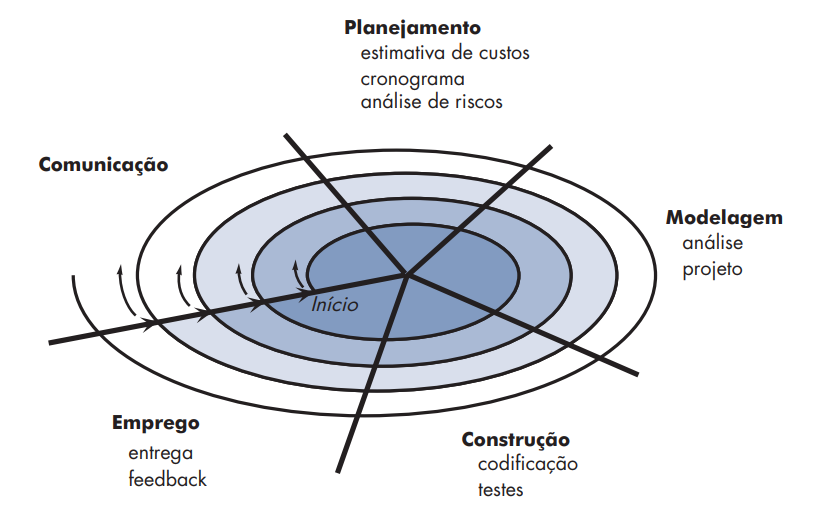
\includegraphics[width=0.9\linewidth]{figuras/spiral-model.png}
    \caption{Ciclo de vida do modelo espiral}
    \label{spiral-model}
\end{figure}
\newpage
Um modelo espiral é dividido em um conjunto de atividades metodológicas, cada uma dessas atividades representa um segmento do caminho espiral ilustrado na Figura \ref{spiral-model}. Diferente de outros modelos de processo, que terminam quando o software é entregue, o modelo espiral pode ser adaptado para ser aplicado ao longo de todo ciclo de vida do software.

O primeiro circuito em torno da espiral pode representar um “projeto de desenvolvimento de conceitos” que começa no núcleo da espiral e continua por várias iterações, até que o desenvolvimento de conceitos esteja completo. Se o conceito for desenvolvido para ser um requisito final, o processo prossegue pela espiral pelas “bordas” e um “novo projeto de desenvolvimento de produto” se inicia \cite{maxim2021engenharia}. As ideias precisavam de validação de usuários. Por isso, a prototipação foi muito utilizada como mecanismo de redução de riscos como o modelo sugere. 

% No modelo evolutivo, como o próprio nome sugere, os requisitos vão evoluindo conforme a aplicação evolui e esse processo ocorre em paralelo à evolução da aplicação. Esse paradigma é muito útil quando o cliente não tem todas as funcionalidades necessárias para a solução. Nesse contexto, foi paradigma que mais se adequou a esse trabalho tendo em vista que nem todos os requisitos eram bem definidos de início. Além disto, as funcionalidades do jogo precisam ser validadas frequentemente uma vez que a jogabilidade precisa ser atraente ao público. Portanto, a cada nova versão foram realizadas reuniões com colegas, e com a orientadora, a fim de receber \textit{feedbacks} que auxiliem na melhoria dos recursos, de modo contínuo.

As atividades realizadas no modelo ilustrado na Figura \ref{spiral-model} são:
\begin{itemize}
    \item \textbf{Planejamento:} A fase de planejamento é a base sobre a qual todo o projeto de desenvolvimento de software deve ser construído. Durante essa fase são definidos os recursos um cronograma e a análise de riscos;
    \item \textbf{Modelagem:} Nessa fase elabora-se um "esboço" do sistema, permitindo uma visão geral de sua estrutura e funcionamento;
    \item \textbf{Construção:} Essa etapa envolve a produção do código e a realização de testes para identificar e corrigir possíveis erros na codificação.;
    \item \textbf{Validação:} Ao chegar nessa etapa, O software, seja como uma solução completa ou como um incremento parcialmente implementado, é entregue ao cliente para avaliação. Com base nessa análise, o cliente fornece \textit{feedback} sobre o produto entregue.
\end{itemize}


\section{\textit{Role-Playing Games} (RPG)}
\label{sec:rpg}

Um \textit{role-playing game} \footnote{Role Playing Game \url{https://en.wikipedia.org/wiki/Role-playing_game}} consiste de um tipo de jogo no qual jogadores assumem papéis de algum domínio proposto e devem atuar de acordo com um sistema de regras definido. Há diversos tipos de RPGs, com regras e estilos bem variados. As seções a seguir exploram alguns estilos de RPG.

\subsection{RPG de Mesa}
\label{sec:rpg-de-mesa}
Em meados de 1974, nos Estados Unidos, foi publicado um jogo chamado \textit{Dungeons} \& \textit{Dragons} \footnote{D\&D - \textit{Dungeons and Dragons} \url{https://dnd.wizards.com/pt-BR}}. Este jogo foi considerado o primeiro RPG com interpretação de papéis e ambientação em um universo de fantasia medieval.

A ideia do jogo \footnote{Básico do Jogo D\&D \url{https://dnd.wizards.com/pt-BR/what-is-dnd/basics-play}} consiste de cada jogador à mesa construir a história, personalidade e ficha de seu personagem. Após isto, o mestre de jogo (ou narrador), que já planejou a história anteriormente, irá dar prosseguimento narrando a história e dando início ao jogo, conduzido pela própria imaginação. Os jogadores jogam dados para determinar quais dos seus ataques acertam e quais erram, se seu personagem percebe ou não uma armadilha escondida; as ações são determinadas através dos dados. Outro elemento do jogo é a ``ficha de personagem'' que consiste de um documento que deve conter as características que definem os detalhes necessários do personagem de um jogador. Esta ficha determina o quão habilidoso seu personagem é em fazer determinadas ações. Já a história refere-se a um plano de fundo que o jogador inventa para o seu personagem com o intuito de contribuir para um jogo rico em detalhes. 

\subsection{RPG Eletrônico}
\label{sec:rpg-eletronico}
Após o sucesso dos RPGs de mesa, e com o avanço da tecnologia, esse estilo de jogo saiu das mesas e chegou aos computadores e consoles, deixando de depender totalmente da imaginação, já que os computadores passaram a renderizar gráficos cada vez melhores e mais realistas. Esse estilo de jogo se popularizou e atualmente é um dos gêneros de jogos mais populares segundo a NEWZOO \cite{NEWZOO}.

Atualmente, os RPGs giram em torno de um universo fictício chamado \textit{ambientação} que pode ser medieval, ocidental, espacial, realista ou qualquer outro que a imaginação conceber. Esse universo forma o cenário onde os personagens interagem e constroem sua história, profissão, cultura e tecnologias \cite{duflo1999jogo}.

\subsection{O RPG na Educação}
\label{sec:rpg-na-educacao}
Esse gênero de jogo tem se destacado não apenas no video-game, mas também como ferramentas versáteis com aplicações em diversas áreas. Caracterizados pela imersão em narrativas interativas e pela personalização de personagens, esses jogos já foram utilizados em diversas áreas fora o entretenimento e tiveram resultados positivos. Por exemplo, na UFG (universidade de Goiás), foi desenvolvido um jogo RPG para os cursos de Ciências e Biologia (\cite{soares2016role}) com o objetivo de mediar a aprendizagem, diversificar e avaliar a transmissão do conhecimento. O jogo consiste de uma aventura dentro do corpo humano com 25 questões a respeito de Fisiologia Humana Básica, os alunos do curso demonstram grande interesse pelo jogo e aprovaram o modelo didático e perceberam sua eficácia ao associar a imaginação e a forma como pode ser utilizado para ensinar e avaliar os conhecimentos adquiridos.


%  ================================ 2.2 Princípios de Game Design ================================
% 

% =================== PYGAME-CE =======================================
\section{Desenvolvimento de Jogos}
\label{sec-desenvolvimento-de-jogos}
Um jogo eletrônico é um tipo de aplicativo que normalmente é usado para fins de entretenimento, mas também pode ser projetado para objetivos mais sérios, com potencial de aplicação em diversas áreas, como por exemplo educação, negócios e saúde. Desenvolver um jogo é uma tarefa desafiadora devido às diversas atividades multidisciplinares envolvidas, tornando o processo altamente complexo, como discutido nas seções a seguir. 

\subsection{Princípios de Game Design}
\label{sec:principios-de-game-design}
O processo de aprendizagem envolvido na criação e no desenvolvimento de jogos integra uma ampla variedade de conhecimentos. Para criar um jogo, é fundamental ter conhecimento não apenas a programação, mas também áreas como Música, Desenho, inglês, Geometria, Física, Matemática, Lógica, Geografia e Linguagens que se tornam indispensáveis, pois o desenvolvimento de um jogo exige o domínio de programação, design gráfico, efeitos sonoros, criação de fases (\textit{level design}), elaboração de histórias e narrativas (\textit{storytelling}), temática e contextualização \cite{cestari2022aprendizagem}.

Nos primeiros dias do desenvolvimento de videogames, os jogos eram criados por grupos pequenos de pessoas; porém, com o aumento da complexidade dos jogos e a indústria identificando oportunidades promissoras, as equipes eventualmente foram acompanhando o ritmo e a especialização está se tornando cada vez mais necessária à medida que os jogos se tornam maiores. Atualmente, uma equipe de desenvolvimento de jogos engloba profissionais multidisciplinares, cada um com um foco especifico para a produção do jogo. Scott Rogers cita em seu livro \cite{GameDesign} as seguintes: 
\begin{itemize}
    \item \textbf{Programador(a):} Responsável pela programação do software do jogo e das ferramentas utilizadas. Também escreve o documento técnico;
    \item \textbf{Artista:} Responsável pela representação visual dos componentes do jogo desde as interfaces aos personagens estipulados no documento técnico;
    \item \textbf{Designer do Jogo:} Cria as ideias e regras que compõem o jogo do conceito até a forma final.
    \item \textbf{Produtor(a): }Responsável por supervisionar toda a equipe de desenvolvimento do jogo;
    \item \textbf{Testador:} Responsável por jogar constantemente o jogo e relatar problemas ou \textit{bugs} encontrados;
    \item \textbf{Compositor:} Aquele responsável por criar temas e tilhas marcantes que sejam capazes de compor o cenário do jogo e passar os sentimentos que o designer do jogo estipulou;
    \item \textbf{Designer de Som:} Cria todos os efeitos sonoros que são usados em um jogo;
    \item \textbf{Roteirista:}  Responsável por escrever o manual do jogo e qualquer material de suporte fictício, como  biografias de personagens;
    \item \textbf{Gerente de produto:} Um gerente de produto trabalha com a equipe de desenvolvimento e os gerencia com base no cronograma de produção;
    \item \textbf{Diretor Criativo:} É responsável por toda a gestão criativa de uma marca ou projeto;
    \item \textbf{Diretor(a) de Arte:} Responsável por ajudar a equipe a criar um estilo visual do jogo e trabalham com as equipes de marketing a fim de criar os designs dos produtos;
    \item \textbf{Diretor(a) Técnico:} Revisam e recomendam ferramentas e softwares para equipes para ajudá-las a trabalhar de forma mais eficiente. Eles fornecem suporte técnico e aconselhamento quando há deficiências na equipe.
\end{itemize}

Em um jogo com finalidade pedagógica, é essencial não esquecer de incluir elementos a favor da diversão e do entretenimento utilizando o melhor de todas as áreas citadas anteriormente para essa finalidade. Muitos jogos educacionais infringem este princípio por se preocuparem demais com as questões escolares. Com isso, o jogo se torna chato e o seu propósito não é alcançado. É necessário unir o elemento educacional ao entretenimento para alcançar o objetivo de forma equilibrada.

\subsection{\textit{Game Loop}}
\label{sec:game-loop}
Jogos eletrônicos consistem de uma sequência de pegar a entrada do usuário, atualizar o estado do jogo, lidar com a IA, tocar música e efeitos sonoros, e mostrar o jogo na tela. Esta sequência é feita através do \textit{game loop}. Basicamente o \textit{game loop} é o ''batimento cardíaco do jogo''. Cada iteração do loop corresponde a um \textit{frame} (quadro) do jogo, \footnote{Python Brasil \url{https://wiki.python.org.br/GameLoop#:~:text="game%20loop".-,O%20"Game%20Loop",batimento%20cardíaco%20de%20cada%20jogo.}}.

A figura \ref{fig:event-loop} ilustra um \textit{loop} de jogo com os três elementos básicos fundamentais, que são executados continuamente a cada volta do loop durante o jogo \footnote{Game Programming Patterns \url{https://gameprogrammingpatterns.com/game-loop.html}}.


\begin{figure}[h!]
    \centering
    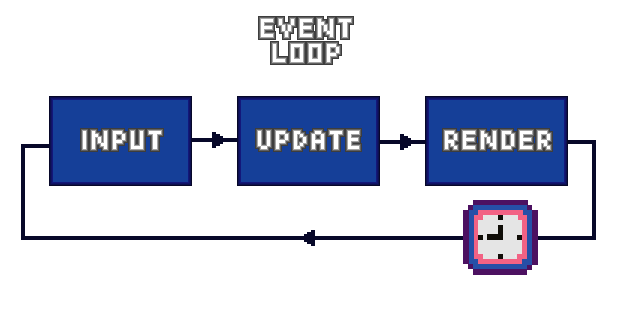
\includegraphics[width=1\linewidth]{figuras/event-loop.png}
    \caption{\textit{Event Loop}}
    \label{fig:event-loop}
\end{figure}

\begin{itemize}
    \item \textit{\textbf{Input:}} Processa a entrada do usuário sem bloqueio;
    \item \textit{\textbf{Update:}} Atualiza o estado do jogo;
    \item \textit{\textbf{Render:}}  Desenha o jogo;
    \item \textit{\textbf{Delta time:}} O relógio na figura simboliza que este loop é executado a uma velocidade constante. Será explicada a seguir. 
\end{itemize}

% Delta time
\subsection{Delta Time}
\label{sec:delta-time}
Nos primeiros videogames, os programadores sabiam exatamente qual hardware executaria o jogo que estavam codificando. O código era escrito especificamente para aquele dispositivo e cuidadosamente projetado para realizar apenas o trabalho necessário em cada quadro, garantindo que o jogo rodasse na velocidade desejada pelos desenvolvedores.
Atualmente é pouco provável saber em qual hardware o jogo será executado, ou seja, quando estivermos codificando um jogo temos que fazer ele se adaptar de forma inteligente a diversos dispositivos.

 Para resolver esse problema, o \textit{Delta time} (diferença de tempo) tornou-se um padrão amplamente utilizado na maioria dos jogos. Ela consiste de uma variável numérica que armazena a diferença entre o último \textit{clock} do processador (\textit{t'}) e o \textit{clock} atual (\textit{t}), como mostrado na equação a seguir.
 \begin{equation}
    \Delta t = t' - t
    \label{eq:dt_equation}
\end{equation}

Supondo que tenhamos dois computadores diferentes para executar o jogo, um potente que consiga rodar a 120 FPS (\textit{frames per second}) quadros por segundo e outro menos potente que execute a 30 FPS. Supondo que a velocidade de movimento seja 1 unidade. Sem o delta time o movimento seria da seguinte forma:
\begin{itemize}
    \item \textbf{Computador Potente:} 1 unidade x 120 quadros = 120 unidades de movimento por segundo.
    \item \textbf{Computador Lento:} 1 unidade x 30 quadros = 30 unidades de movimento por segundo.
\end{itemize}

Se assim fosse feito, o jogador do computador potente se moveria quatro vezes mais rápido em relação ao jogador do computador lento, os jogos seriam injustos e inconsistentes. Veja agora como é feito com o \textit{delta time}.
\begin{itemize}
    \item \textbf{Computador Potente (120FPS):} \( \Delta = \frac{1}{120}\) = 0.0083 
    
    0.0083 x 120 quadros \begin{math} \approx\end{math} 1 unidade.
    \item \textbf{Computador Lento (30FPS):} \( \Delta = \frac{1}{30}\) = 0.0333 
    
    0.0333 x 30 quadros \begin{math} \approx\end{math} 1 unidade.
\end{itemize}

Esse valor é usado para ajustar todas as operações dependentes de tempo, como movimento ou animações.

 % Quando dizemos que um jogo roda a 30 FPS (\textit{frames per second}) quadros por segundo, queremos dizer que o \textit{game loop} é executado 30 vezes por segundo, temos o valor de delta como \(\frac{1}{30}\), o que significa dizer que o \textit{game loop} do jogo leva \(\frac{1}{30}\) segundos para ser executado. Essa informação é utilizada para resolver o problema introduzido pela evolução dos computadores que, hoje, são extremamente mais velozes hoje do que nas décadas de 80 e 90. Jogos desenvolvidos nesta época não rodariam nas máquinas atuais sem um controle temporal do \textit{delta time}. 
 
 % , e se um computador atual executasse um jogo dos anos 80 hoje sem nenhum mecanismo de controle, o jogo rodaria a alguns milhares de quadros e a experiência não seria boa se não fosse utilizado desse \textit{pattern} de jogos, não existiria uma normalidade entre dispositivos.
 
\subsection{Pygame-ce}
\label{sec:pygame-ce}
Pygame-ce (Community Edition) \footnote{https://github.com/pygame-community/pygame-ce/} é uma biblioteca multiplataforma gratuita e de código aberto que surgiu de um \textit{fork} do projeto \textit{Pygame} por seus antigos desenvolvedores principais. Seu foco é construir aplicativos multimídia como videogames utilizando a linguagem Python. A biblioteca está sob a licença GNU LGPL version 2.1, o que significa que pode ser usada em qualquer projeto desde que, se forem feitas quaisquer alterações ou adições ao código-fonte, elas devem ser lançadas com uma licença compatível.

 A Pygame-ce usa a biblioteca SDL (Simple DirectMedia Layer)\footnote{SDL (Simple DirectMedia Layer) \url{https://www.libsdl.org/}} que consiste de uma biblioteca de desenvolvimento multiplataforma também de código aberto e escrita em C, projetada para fornecer acesso de baixo nível a hardware de áudio, teclado, mouse, \textit{joystick} e gráficos via OpenGL e Direct3D além de várias outras bibliotecas populares para abstrair as funções mais comuns. A SDL age como um \textit{wrapper} de camada fina e multiplataforma, fornecendo suporte a operações de pixel 2D, som, acesso à arquivos, manipulação de eventos, temporizadores e \textit{threading}.
As principais funcionalidades da \textit{Pygame} incluem:
\begin{itemize}
    \item Carregamento e exibição de imagens;
    \item Criação de animações e renderização quadros de jogos;
    \item Adição de música de fundo e efeitos sonoros;
    \item Manipulação de dispositivos de entrada;
    \item Gerenciamento de \textit{sprites} através de classes integradas.
\end{itemize}

Como a maioria das bibliotecas de python, \textit{Pygame} pode ser adicionada via \textit{prompt} de comandos do sistema operacional  por meio do pip\footnote{pip \url{https://pip.pypa.io/en/stable/}}. O pip é um sistema de gerenciamento de pacotes para Python, usado para instalar e gerenciar pacotes de software escritos na linguagem de programação Python. Ele simplifica o processo de instalação, atualização e remoção de pacotes e suas dependências.

A listagem a seguir \ref{lst-circle-movement} é apresentado um código básico de Pygame\footnote{Pygame Docs \url{https://pyga.me/docs/}} para desenhar um circulo na tela e movimenta-lo. 
\newpage
\lstinputlisting[label=lst-circle-movement, caption=Exemplo de código Pygame Para Mover um Circulo., language=Python, float=htpb]{codigos/circle_movement.py}
% completar aqui
Na linha (2) é feito a importação do Pygame e dizemos ao compilador para carregar os seus módulos; nas linhas (5) à (8) fazemos a inicialização básica de todo código Pygame onde inicializamos o Pygame configuramos a tela inicial, configuramos as variáveis de controle \textit{clock} e \textit{running}; a linha (11) é definida a posição inicial do círculo, na linha (13) é onde começa o \textit{loop} principal do jogo que consiste em:
\begin{enumerate}
    \item verificar se o jogador fechou o jogo (linhas 16 a 18);
    \item preencher toda a tela com a cor roxa (linha 21);
    \item desenhar o círculo vermelho na posição \textit{player\_pos} (linha 23);
    \item fazer a captura da entrada do jogador (25) e se for o alguma das ("w", "s", "a", "d") move o círculo a respectiva direção (linhas 26 a 33);
    \item a linha (36) atualiza o conteúdo de toda essa exibição;
    \item atualizamos o valor do \textit{delta\_time} como explicado na seção \ref{sec:delta-time} este método que deve ser chamado uma vez por \textit{frame} e retornará quantos milissegundos se passaram desde a chamada anterior, como passamos o valor 60 de parâmetro, o jogo não passará de 60 FPS.
\end{enumerate}
% coisas para explicar?
% colocar um codigo com \href{https://pyga.me/docs/ref/music.html}{pygame.mixer.música} \href{https://pyga.me/docs/ref/draw.html}{pygame.draw} 
% \href{https://pyga.me/docs/ref/event.html}{pygame.event} 
% \href{https://pyga.me/docs/ref/font.html}{pygame.font} 
% \href{https://pyga.me/docs/ref/image.html}{pygame.image} 
% \href{https://pyga.me/docs/ref/key.html}{pygame.key} 
% \href{https://pyga.me/docs/ref/rect.html}{pygame.Rect} 
% \href{https://pyga.me/docs/ref/sprite.html}{pygame.sprite} 
% \href{https://pyga.me/docs/ref/surface.html}{pygame.Surface} 
% \href{https://pyga.me/docs/ref/transform.html}{pygame.transform} 
% \href{https://pyga.me/docs/ref/window.html}{pygame.Window} 
% completar aqui
%  ======================================= 2.3 Mapas =================================

\section{Mapas}
\label{sec-mapas}
% explicar oq e um editor de mapas

Os mapas de jogo desempenham um papel fundamental no design e na experiência de um jogo, servindo como o alicerce do mundo virtual onde a narrativa, os desafios e a exploração ocorrem. Os mapas ajudam a transmitir a ambientação, geografia e lógica do universo do jogo proporcionando imersão e ambientação do jogador. Para a criação de mapas são utilizadas ferramentas que auxiliam nesse processo, esses são os editores de mapas.

 Os softwares editores de mapas permitem o designer do criar de forma visual e intuitiva os mapas de seus jogos. Praticamente todos os jogos usam uma ferramenta para esse propósito, tanto jogos 2D como também jogos 3D. Nesse trabalho  utilizou-se de editor 2D. Um editor de mapas 2D se fundamenta em uma técnica denominada \textit{Tile-Based}, onde o cenário é formado por pequenas imagens quadradas, retangulares ou hexagonais chamados \textit{tiles} (ladrilhos).
% citar jogos populares que utilizam essa técnica (dofus)

\subsection{\textit{Tiles} e \textit{Tilesets}}
\label{sec:tiles-e-tilesets}
\textit{Tilesets} são coleções de pequenas imagens reutilizáveis, chamados \textit{tiles}, organizadas em uma grade. Cada \textit{tile} representa uma pequena parte do mundo de um jogo 2D, como, por exemplo, um pedaço de chão, um segmento de uma parede ou uma decoração. Ao combinar diferentes tiles em diversas posições, cria-se um cenário que pode ser utilizado como fase de um jogo. 

Trata-se de um recurso gráfico para desenhar níveis e outros componentes estáticos de um jogo de forma rápida e eficiente, já que não é necessário desenhar toda a área jogável. Esses \textit{tilesets} podem ser de duas formas: i) \textit{\textbf{top-down}} (cima para baixo) esses tiles são desenhados na perspectiva vista de cima para baixo, alguns jogos que utilizam desse tipo de tile são \textit{The Legend of Zelda} e \textit{Chrono Trigger} veja a figura \ref{fig:tileset-orthogonal}; ii) \textit{\textbf{platformer}} (plataforma) esses tiles são desenhados na perspectiva lateral, utilizada em jogos onde o jogador realiza saltos e desvia de obstáculos, é o caso de jogos, como \textit{Super Mario} e \textit{Sonic} a figura \ref{fig:tileset-platform-orthogonal} ilustra esse tipo de \textit{tile}.

\begin{figure}[h!]
    \centering
    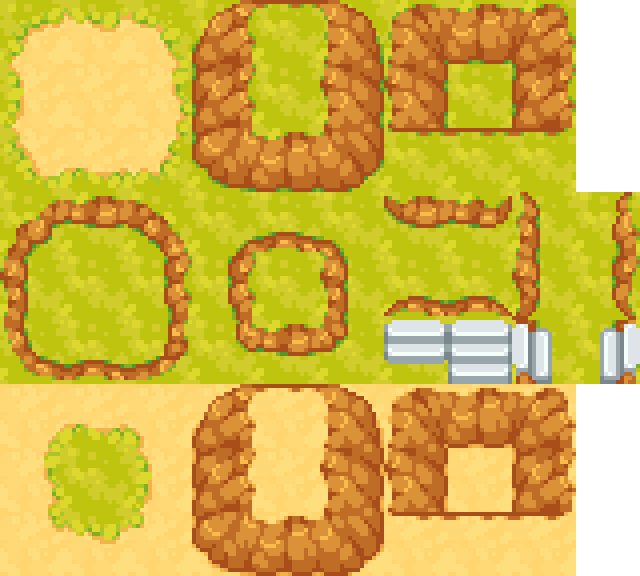
\includegraphics[width=1\linewidth]{figuras/tileset.png}
    \caption{Exemplo de \textit{tileset top-down}}
    \label{fig:tileset-orthogonal}
\end{figure}
\begin{figure}[h!]
    \centering
    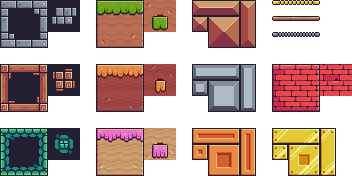
\includegraphics[width=1\linewidth]{figuras/tileset-orthogonal-platform.png}
    \caption{Exemplo de \textit{tileset platformer}}
    \label{fig:tileset-platform-orthogonal}
\end{figure}

\clearpage
\subsection{Tiled}
\label{sec:tiled}
O Tiled \footnote{Tiled \textit{Map Editor} \url{https://www.mapeditor.org}} é um editor de mapas 2D \textit{open source} que ajuda \textit{game designers} a desenvolverem o conteúdo de seus jogos. Seu principal recurso é desenhar e editar mapas de \textit{tiles} de qualquer tamanho, sem restrições quanto ao tamanho dos \textit{tiles}, ao número de camadas ou à forma como os tiles podem ser utilizados.

No software, é possível posicionar \textit{tiles} em ''quadradinhos'' e, aos poucos, o cenário ganha forma, veja a figura \ref{fig:example-tiled}. Esses \textit{tiles} podem ser  retangulares, retas, isométricas projetadas, isométricas escalonadas e hexagonais escalonadas. Tiled Também é capaz adicionar imagens, retângulos, pontos e outras formas geométricas de forma livre ao mapa, bem como adicionar metadados a eles, que poderão futuramente serem usados pelo programador \cite{tiled}. 
\begin{figure}[h!]
    \centering
    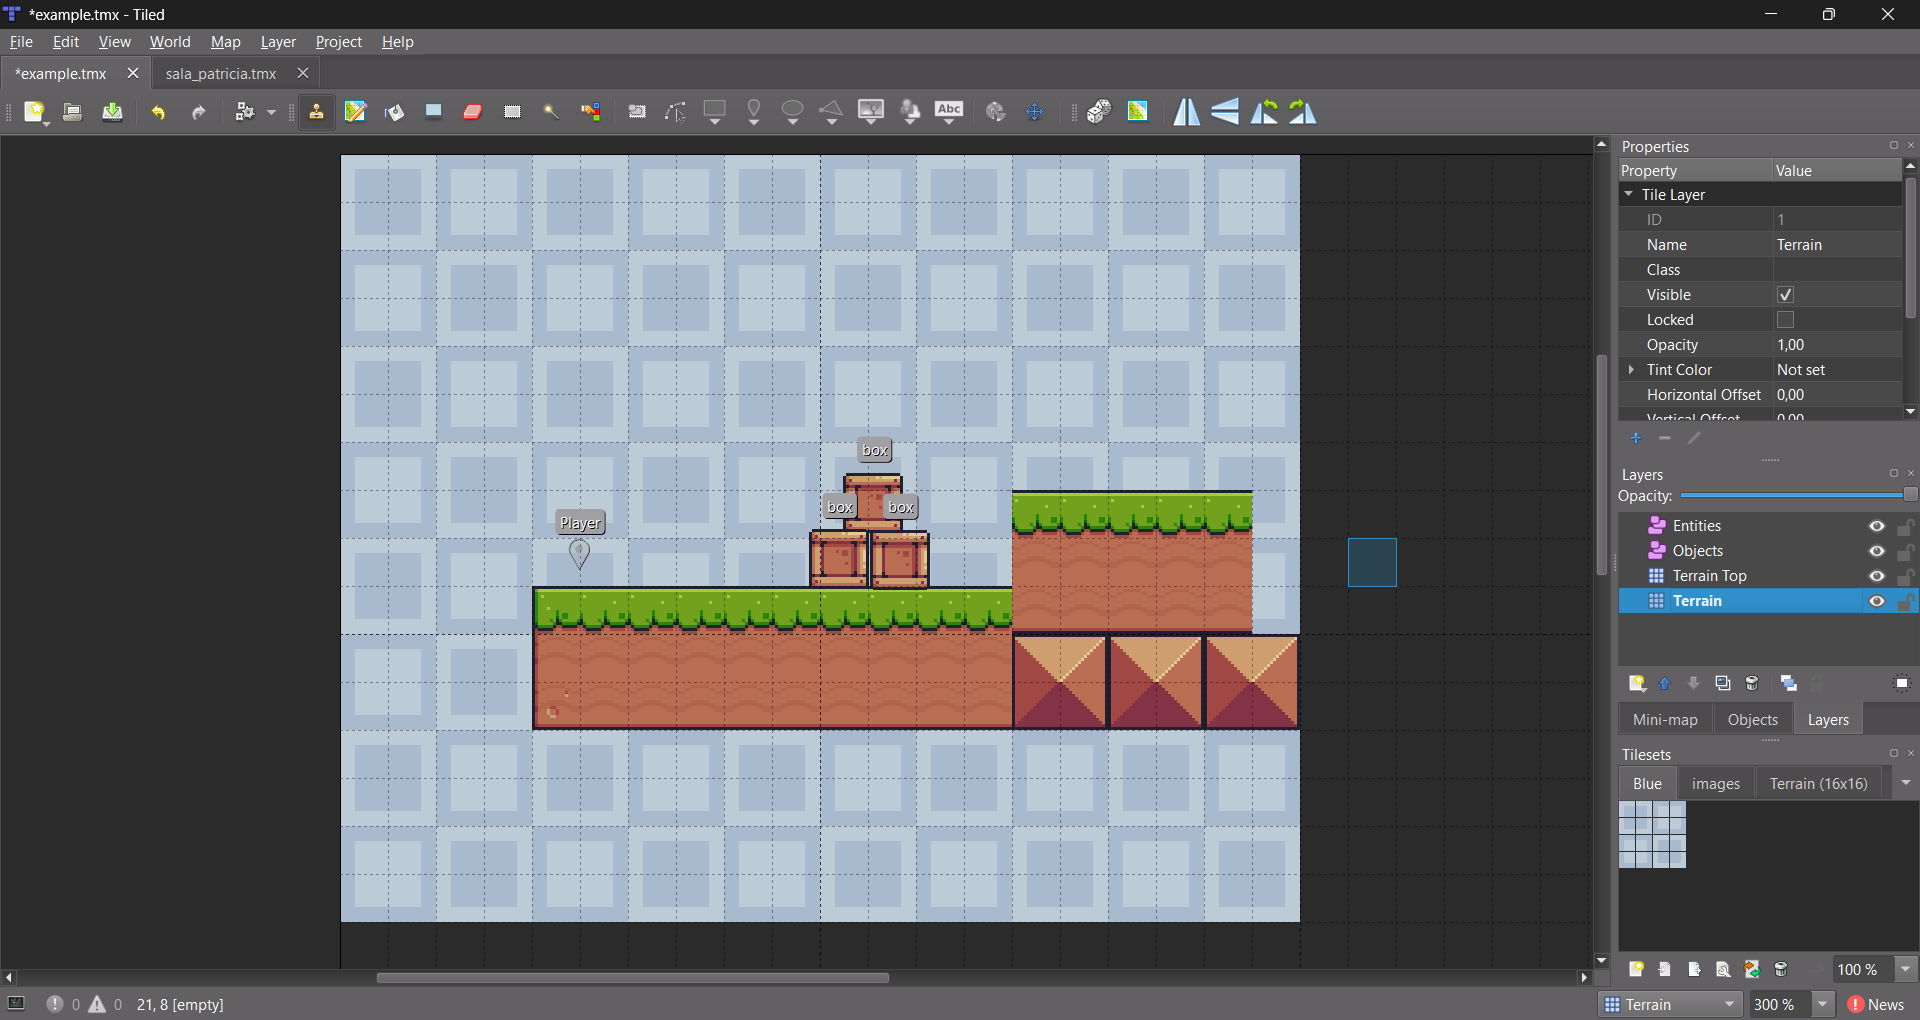
\includegraphics[width=1\linewidth]{figuras/example-tiled.png}
    \caption{Exemplo de criação de mapa no \textit{Tiled} com tiles 16 x 16}
    \label{fig:example-tiled}
\end{figure}

Jogos costumam ter cenários com várias camadas, o Tiled é capaz de trabalhar com camadas de forma similar a outros programas editores de imagens. Ao fazer isso é possível definir a ordem com que os ladrilhos serão renderizados no jogo, sendo o padrão \textit{bottom-up} (de baixo para cima), ou seja, em caso de blocos sobrepostos, o bloco que está em uma camada superior terá prioridade. A figura \ref{fig:layers} ilustra as camadas do mapa da figura anterior sendo elas (i) terreno, (ii) topo do terreno (iii) objetos e (iv) entidades. 
\clearpage
\begin{figure}[h!]
    \centering
    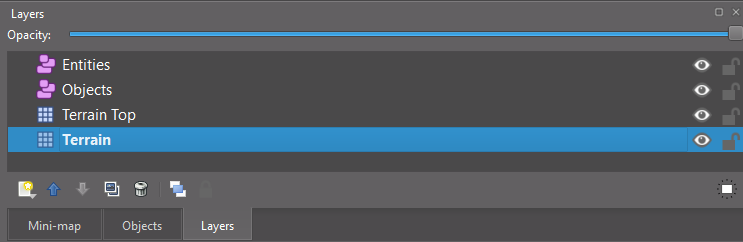
\includegraphics[width=1\linewidth]{figuras/layers.png}
    \caption{Camadas no Tiled}
    \label{fig:layers}
\end{figure}

Existem 4 possíveis tipos de camadas no Tiled, duas delas utilizadas nesse tela: 
\begin{itemize}
    \item \textbf{(i) Camada de tiles}: Nessa camada que é feito o posicionamento de \textit{tiles}. São as camadas ``\textit{Terrain}'' e ``\textit{Terrain} Top'' da figura \ref{fig:layers};
    \item \textbf{(ii) Camada de objetos}  Nessa camada é permitido posicionar objetos, imagens, retângulos formas geométricas entre outros, sem a necessidade de posicionar na grade específica do software. É nessa camada que são adicionados metadados aos objetos nelas. São as camadas``\textit{Entities}'' e ``\textit{Objects}'' da figura \ref{fig:layers}.
\end{itemize}


%  ======================================= PyTMX =======================================
Após a criação do mapa, o programa é capaz de exportar o conteúdo para diversos formatos compatíveis com diferentes bibliotecas \footnote{Bibliotecas e \textit{frameworks} compatíveis com o Tiled \url{https://doc.mapeditor.org/en/stable/reference/support-for-tmx-maps/}}. Nesse trabalho foi utilizado o formato TMX \textit{(Translation Memory eXchange)}, esse formato se assemelha a um XML \textit{ (Extensible Markup Language)}, por ser composto de \textit{tags} e atributos que podem ser recuperadas pelo programador.

% , e  (batalha naval) que é como o mapa é feito pelo programa acrônimo de Translation Memory eXchange, é um formato baseado no 'xml' devido a isso faz o uso de tags e atributos de arquivo padrão usado na indústria de tradução para armazenar e trocar memórias de tradução, basicamente consiste em uma seção de cabeçalho, seguido por uma ou várias seções de corpo, cada uma contendo unidades de tradução

\subsection{PyTMX}
\label{sec:pytmx}
PyTMX é uma biblioteca de código aberto escrita para a linguagem Python e projetada para desenvolvimento de jogos \footnote{PyTMX \url{https://pytmx.readthedocs.io/en/latest/}}.. Sua principal função é carregar mapas e seus dados para o programa.

O software suporta o carregamento inteligente de tiles, utilizando uma base de armazenamento rápida e eficiente. No PyTMX, é possível manipular a maioria dos tipos de objetos do Tiled, incluindo metadados. Isso permite modificar mapas e objetos diretamente no Tiled, sem a necessidade de alterar o código-fonte. A Listagem \ref{lst-load-map} mostra como é feita a importação de um mapa feito no Tiled para o Pygame.

\clearpage
\lstinputlisting[label=lst-load-map, caption=Exemplo de utilização da biblioteca Pytmx, language=Python, float=htpb]{codigos/load_map.py}

Na linha (7) da listagem anterior é carregado todo o conteúdo do mapa para a variável \textit{tiled\_map}. Com isso é possível recuperar informações que estão no mapa como, objetos, posição, tamanho e propriedades. 


%  ======================================= Pixel Art ===================================
\section{Pixel Art}
\label{sec:pixel-art}
O termo \textit{pixel}, originado das palavras \textit{picture} e \textit{element} (elemento de imagem), refere-se à menor  unidade de uma imagem que pode ser expressa digitalmente \cite{lyon2006brief}. A \textit{Pixel Art} consiste de um tipo de arte que usa \textit{pixels} visíveis para compor uma image, formada pela junção de diversos pontos digitais.

A \textit{Pixel Art} surgiu nos anos 1960, mas foi popularizada nos anos 1970 e 1980. Nessa época de início dessas tecnologia, os monitores ainda não possuíam a alta quantidade de pixels presente nos dispositivos atuais. Era necessário desenhar objetos na tela com ''quadradinhos'' uma vez que era o único recurso que da época. Contudo, até nos dias atuais, é um estilo de arte amplamente apreciado. Na figura abaixo vemos alguns exemplos de Pixel Art de diferentes épocas.

\begin{figure}[h!]
    \centering
    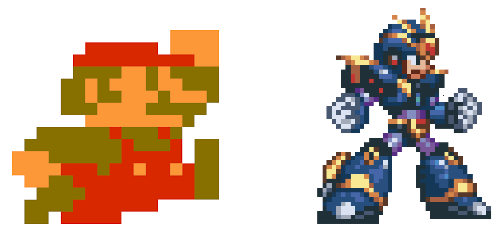
\includegraphics[width=0.6\linewidth]{figuras/comparative-8bit-32-bit-pixel-art.png}
    \caption{Figura ilustrando a esquerda o Super Mario Bros 1985, e a direita o Mega Man 1998}
    \label{fig:enter-label}
\end{figure}

\subsection{Aseprite}  
\label{sec:aseprite}
O Aseprite\footnote{Aseprite \url{https://www.aseprite.org}} é um software comercial especializado em Pixel Art que oferece recursos e ferramentas específicas para essa finalidade, permitindo assim a criação de \textit{sprites} e animações 2D para videogames. As ferramentas de Aseprite permitem controlar a animação quadro a quadro realizar rotações de Pixel Art previamente desenvolvidas.
A figura \ref{fig:aseprite} ilustra a tela básica do programa. À primeira, vista ele é semelhante a outros \textit{softwares} de criação de imagens, exceto pela sua grade quadriculada.  
\begin{figure}[h!]
    \centering
    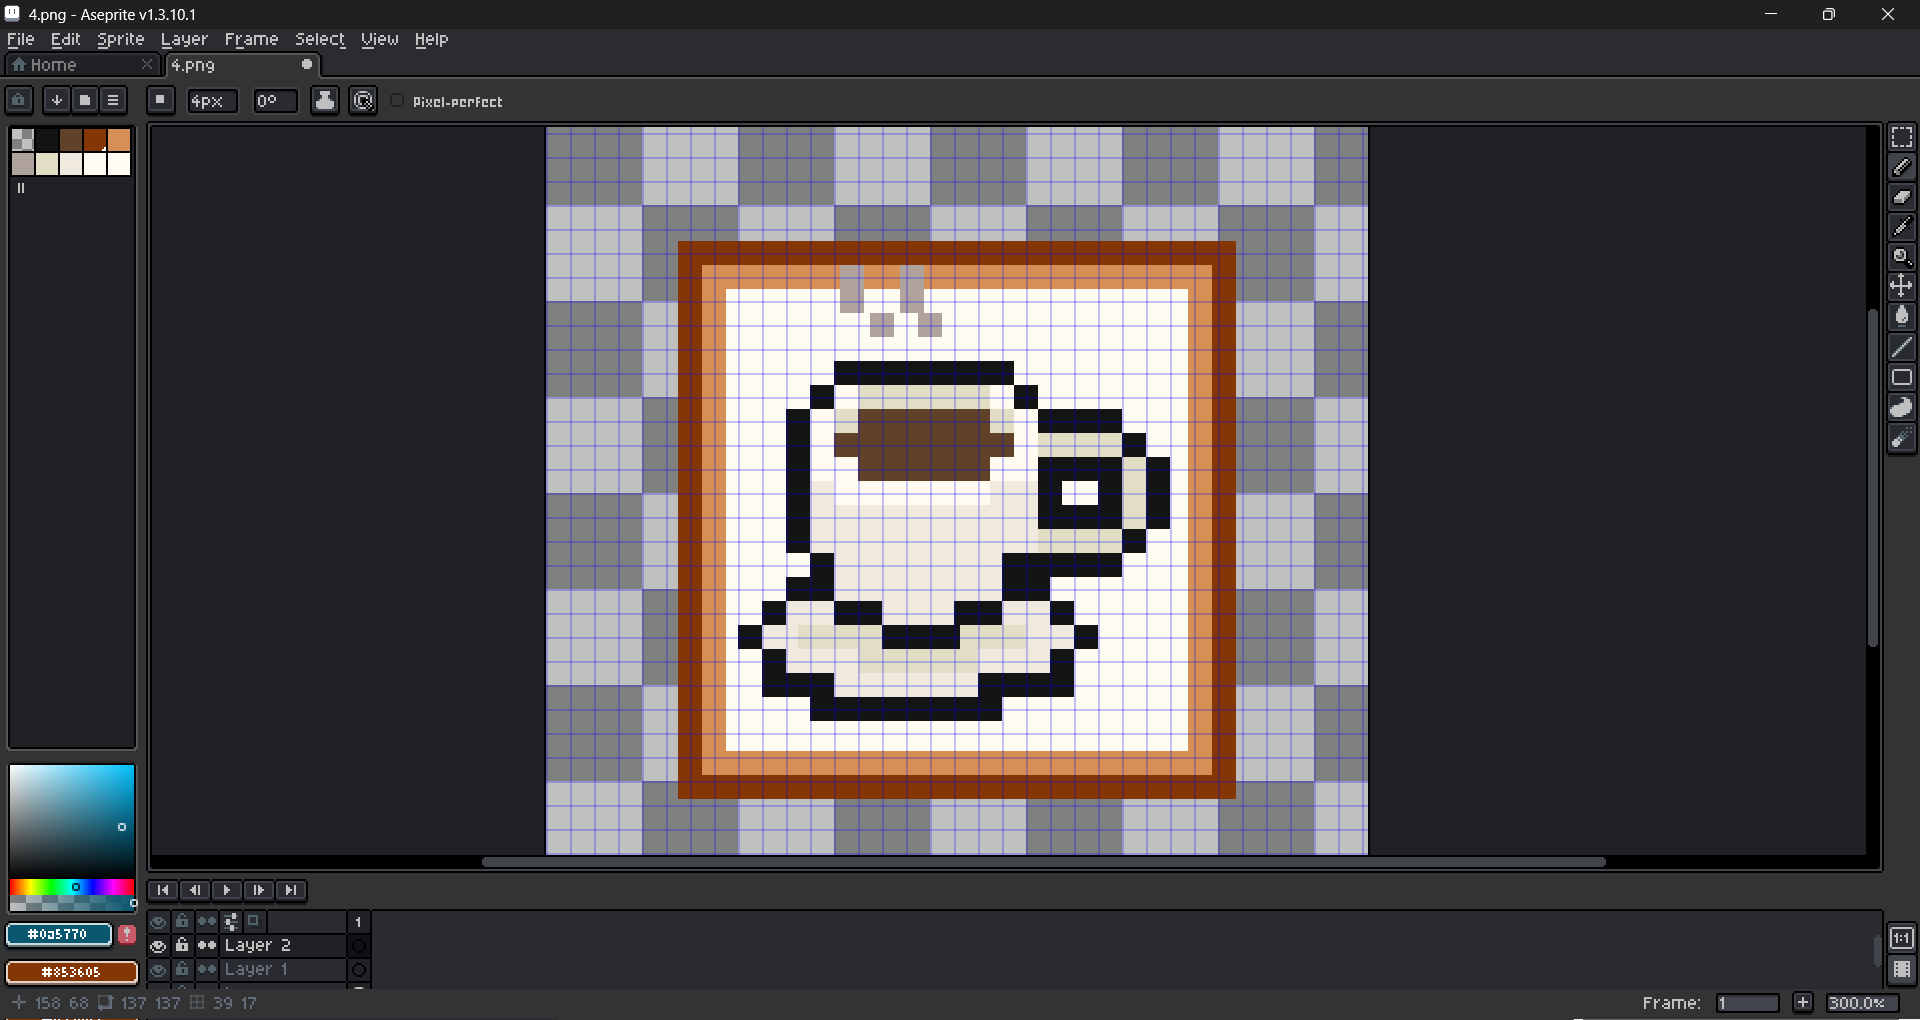
\includegraphics[width=1\linewidth]{figuras/aseprite.png}
    \caption{Visão básica do software Aseprite}
    \label{fig:aseprite}
\end{figure}

% Um \textit{Sprite} é um objeto gráfico bidimensional (2D) usado em computação gráfica e, particularmente, em videogames.
Um \textit{sprite} normalmente consiste de uma imagem de \textit{bitmap} ou uma série de imagens que são combinadas para criar uma animação. Especificamente no Aseprite, um \textit{sprite} consiste em uma sequência de quadros somados em uma pilha de camadas. A intersecção de quadros e camadas cria uma matriz de células gráficas editáveis com imagens/pixels que podem ser editados com o editor de \textit{sprites} . Camadas, quadros e células são visíveis na linha do tempo.

A figura abaixo ilustra um exemplo de \textit{sprite} de personagem com animação de corrida. Para criar o efeito de movimento, cada uma das imagens é alternada em uma determinada velocidade, produzindo a impressão de movimento.

\begin{figure}[h!]
    \centering
    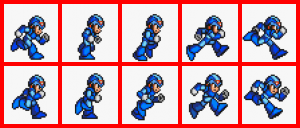
\includegraphics[width=1\linewidth]{figuras/megaman-sprite-animation-export.png}
    \caption{Sprite de movimento do Mega Man (área desenhada de vermelha somente de referencia)}
    \label{fig:sprite-animation}
\end{figure}
% \begin{figure}[h!]
%     \centering
%     
\includegraphics[width=1\linewidth]{figuras/sprite-frog.png}
%     \caption{Ninja Frog exemplo de\textit{sprite}}
%     \label{fig:sprite-frog}
% \end{figure}



% \subsection{Animação}
% \label{sec:animacao}
% A simulação de movimento criada por uma série de imagens é denominada animação. O olho humano  consegue reter uma imagem por aproximadamente 1/10 de segundo

%  A animação é a ilusão de movimento que nossos cérebros nos enganam para perceber quando vemos vários quadros de obras de arte estáticos reproduzidos em rápida sucessão.
% Um quadro é uma única imagem estática em um sprite, se adicionarmos e alterarmos os quadros a uma certa velocidade, cria-se a a impressão de movimento, ao qual dá-se o nome de Animação. 
% Em programação existem várias formas de fazer a animação e uma delas é através de vetores, essa técnica consiste em carregar uma imagem e dizermos ao computador que queremos dividir essa imagem e armazena-lo num vetor. A figura \ref{fig:sprite-animation} exemplifica isso, nesse caso um vetor de duas linhas e cinco colunas, assim para fazer a animação desse personagem, basta percorrer as imagens de forma alternada enquanto capturamos a entrada do jogador e vemos se é movimento








